\section{实验主要方法}
% 实验方法
%% [x] 视觉刺激与行为范式
%% [x] 行为学结果分析
%% [ ] 电极定位
%% [x] 能量谱分析
%% [x] 能量曲线
%% [ ] 支持向量机
%% [ ] 相位分析
%% [x] 代码的获取

\subsection{视觉刺激与行为范式}

我们利用自制的Python程序, 依托PsychoPy软件\cite{psychopy}实时生成视觉刺激。
刺激主体为移动光栅(drifting grating), 每次视觉刺激持续1秒钟;
光栅为方波光栅, 对比度为100\%, 时间频率为2Hz, 空间频率为0.05周期每度(cycles per degree)。

我们共设计了3种行为范式, 分别为“轻拍手”, “默想”, 和“空想”(图\ref{fig:human_behavior}~a)。
“轻拍手“范式要求患者主动预判视觉刺激出现的时刻, 并尽可能地在视觉出现前轻按电脑的空格键以记录患者的预判时间。
“默想”范式要求患者主动预判时间刺激的时刻, 但无需做出行为而只需要在脑海中默念。
“空想”范式要求患者放空思想, 以尽量减少主观思考和注意力的影响, 但其视线中心仍需保持在屏幕上。

每种范式又分别有两种时间间隔, 分别为5秒和10秒;
对于5秒间隔, 视觉刺激持续1秒, 50\%灰背景持续4秒;
对于10秒间隔, 视觉刺激持续1秒, 50\%灰背景持续9秒。
每种范式和每个时间间隔刺激均为20次, 刺激结束前后均有20秒的50\%灰背景。

每位患者每天只进行一次实验, 每次的顺序均为“轻拍手”, “默想”, 和“空想”范式,
每个范式均为先10秒间隔后5秒间隔, 两次间隔间有约30到60秒的休息时间。

\subsection{行为学数据分析}

\subsubsection{韦伯定律}
为了量化实验对象的行为学, 同时消除不同时间间隔间的差异,
我们计算了行为学的韦伯系数(Weber's Coefficient)\cite{gibbon1977scalar, hardy2018encoding}。具体公式如下:
\begin{equation}
    W = \frac{\sqrt{\frac{1}{N} \sum_{i=1}^N (x_i - \mu) ^ 2}}{\mu},\ \mathrm{where}\ \mu = \frac{1}{N} \sum_{i=1}^N x_i
\end{equation}
其中, N表示所观察的测试总次数, x为每次轻拍手与前一次光栅刺激开始的相对时间, 反应了患者需要主动计时的时间长度,
即$ x = t_{tapping} - t_{previous\ grating\ onset} $。

韦伯系数的大小可以体现被试行为学测试的准确度, 在这里体现为对时间间隔预测的误差范围。
同时根据韦伯定律, 同类型不同刺激强度的范式的韦伯系数应当一致;
在这里体现为5秒范式和10秒范式的韦伯系数之间的比较, 依据韦伯定律, 两者应当没有统计学差异。

\subsubsection{行为分布图}
为了更细致的体现患者行为中可能存在的学习过程, 我们对行为的分布做了进一步的分析。
我们计算了每次轻拍手的时刻与相应光栅出现时刻的差值作为行为分布图分析用的数据集, 即$\Delta t = t_{tapping} - t_{grating\ onset}$。
我们将前后相邻的两次行为作为一组数据, 前一次轻拍手的时刻作为横轴, 后一次轻拍手的时刻作为竖轴。
对于每一天的一个时间间隔而言, 共有19对这样的数据。我们将19对数据如上述分成了5份(第一份为3对, 其余为4对)。
为了减少偶发事件对分析的影响, 我们将7天相对应的每份合并在一起; 即第一份共有21对, 其余4份各有28对。

不同象限可以反应当时患者行为的不同状态。第一象限表示测试对象出现连续两次延后于光栅的轻拍手;
第三象限表示被试出现连续两次提前于光栅的轻拍手;
而第二、四象限则提示被试两次轻拍手各有一个在光栅前和后。

\subsection{脑电数据处理}

\subsubsection{电极通道定位}

每个电极通道在脑中的定位主要依靠术前的MRI和术后的CT成像(影像数据由华山医院提供)。
我们首先利用FSL程序\cite{fsl}将影像配准到MNI标准空间, 并手动标记每个电极的位置。
我们再利用MNI空间至Talairach空间转换公式\cite{bioelectromagnetism}
获得电极通道相对应的Talairach座标。
之后再利用Talairach Daemon软件\cite{talairach_daemon}获得每个通道相对应的脑区位置。
为进一步方便分析, 我们将各个脑区再根据各自的生理功能大致做了合并。

\subsubsection{能量谱分析}

我们使用自制的Python3程序, 利用scipy\cite{scipy}与numpy\cite{numpy,oliphant2007python}对原始SEEG数据进行后续分析处理。
我们首先将原始数据以时间刺激开始的时刻作为原点, 前后各3秒(5秒间隔)或6秒(10秒间隔)进行切割。
之后, 对各个片段做以复数形式Morlet小波为基础的小波变换。
\begin{equation}
    %def morlet(F, fs):
    %   """Morlet wavelet"""
    %   wtime = np.linspace(-1, 1, 2*fs)
    %   s = 6 / (2 * np.pi * F)
    %   wavelet = np.exp(2*1j*np.pi*wtime*F) * np.exp(-wtime**2/(2*s**2))
    %   return wavelet
    M(f, t) = e ^ {2 \pi f t i} \cdot e ^ {-\frac{t^2}{2 * (6 / 2 \pi f)^2}}
\end{equation}
其中f为小波的震荡频率, t为相对应的时刻点; t的取值范围为-1到1秒, 间隔为0.0005秒。
震荡频率f的变换范围为对数分布的1到150Hz, 共计40个频率点。
将变换后的绝对值的对数形式做Z score标准化, 选取刺激前的3秒到刺激前的1秒作为基线计算标准化所需要的均值与方差;
并将当天标准化后的数值平均后作为能量谱进行做图。

\subsubsection{能量曲线分析}
为了方便后续的量化分析, 并进一步了解特定波段范围脑电, 我们对脑电的能量曲线做了分析。
我们首先对原始数据依照相应的频段范围进行了带通滤波, 主要为$\gamma$波段(30-80 Hz)。
对于带通滤波, 我们选用了有限冲激响应滤波(finite impulse response filter)。
对于滤波后的数据, 再经过了Hilbert转换, 将常量数据转换为以下形式:
\begin{equation}
    S(t) = A(t) \cdot e^{i \theta(t)}
\end{equation}
其中S为变换后的数据, $A$和$\theta$为欧拉形式的两个参数, t为相应的时刻点。
能量的定义为:
\begin{equation}
    u(t) = 10 \cdot \log_{10}(A(t) ^ 2)
\end{equation}
其物理单位为分贝(dB)。将变换后得到的能量曲线做Z score标准化处理,
选取刺激前的3秒到刺激前的1秒作为基线计算标准化所需要的均值与方差。
标准化后的曲线即为相对应波段的能量曲线。

由于所选频率范围属于较高频率, 我们对标准化后的能量曲线做了进一步的
平滑化处理, 处理方式为:
\begin{equation}
    u'(t) = (u * w)(t) = \int_0^t u(\tau) w(t - \tau)\ d \tau
\end{equation}
其中, w为平滑化的核函数; 这里我们选用了高斯函数作为核函数:
\begin{equation}
    w(x) = \frac{1}{\sigma \sqrt{2 \pi}} \exp(- \frac{x^2}{2 \sigma^2})
\end{equation}
其中, \(\sigma\)为核函数的参数, 我们在这里选用了0.05。

% \subsubsection{回现(entrain)与光反应的自动检测}
%
% 原始数据首先通过FIR带通滤波对每个病人和特定脑区特征的频段进行滤波。
% 滤波后的信号进一步通过Hilbert转化并进行了如上述的切割。
% 将变换后的绝对值的对数形式做Z score标准化, 并将当天标准化后的值平均后作为其特征波段的能量值(power)。
%
% 只有在有效窗口(刺激开始的时刻前后1秒或2秒)内能量值大于1.96,
% 同时在非有效窗口的能量值小于1.96的通道或者试验才能被认为有光反应或出现了回现(entrain)。
%
% \subsubsection{回现(entrain)的随机水平(chance level)}
%
% 我们将同一范式, 两次间隔试验的间隔作为基线(时长约为30到60秒)。
% 而后, 我们随机生成1000个刺激起始时刻, 重复上述的自动检测。
% 被认定为有出现了回现的次数占总测试次数的比例即为回现的随机水平。


\subsubsection{相位分析}
相位也是脑电信号的重要组成部分之一。为了量化患者脑电信号的相位,
我们选择了计算脑电信号的ITPC(Inter Trial Phase Cluster)值\cite{gu2010phase}。
计算公式为:
\begin{equation}
    % ITPC = \left\| \frac{\sum_{k=1}^N e^{i \theta_k}}{N} \right\|
    ITPC(t) = \frac{1}{N} \left\| \sum_{k=1}^N e^{i \theta_k(t)} \right\|
\end{equation}
其中N为所观察的测试总次数, $\theta$为Hilbert转换后的欧拉形式参数, t为相对应的时刻点。

% Although ITPC is a mathematically straightforward method,
% it is less commonly applied in the cognitive electrophysiology literature.
% Therefore, you should justify why you included ITPC in the analyses.
% Typically, ITPC is used to investigate the timing and consistency of the timing
% of frequency-band-specific activity because ITPC has more frequency-band specific- ity
% compared to the ERP (this is shown and further discussed in chapter 20).
% Including the details of this analysis in your Methods section involves simply including
% equation 19.1 and perhaps explaining that ITPC is bound by 0 and 1,
% with 0 indicating random phases and 1 indicating perfect phase clustering.
% However, be clear about the term you use for this analysis because in the literature
% you will find the same terms used for different analyses
% (issues of terminology are discussed in sections 21.1 and 37.10).
% The wITPCz is not a commonly used technique, so it should be explained in more detail,
% including how the distribution of wITPC values under the null hypothesis was generated.

ITPC体现了多次刺激间脑电信号的相位集中趋势。根据公式可知, ITPC值的取值范围为0到1。
当ITPC为0时, 提示多次的相位完全随机; 而当ITPC为1时, 提示多次的相位完全相同。

\subsubsection{支持向量机(support vector machine, SVM)分析}
为了进一步量化神经元群体和不同脑区间对时间间隔的编码,
我们利用径向基核函数多分类支持向量机进行评估(multiclass radial-basis function kernel support vector machine )。
我们将时间间隔分割为20份(对于5秒间隔, 每份为250毫秒)。
SVM的实现依赖于LIBSVM库\cite{chang2011libsvm}。
多分类采用了one-against-one的方法, SVM的输出为一个20维的向量, 代表了SVM对于输入数据与对应的20个时刻的相似程度。
SVM的训练与测试采用了留一交叉验证(Leave-One-Out Cross Validation)的方法, 对最后的SVM结果利用Pearson相关系数来做量化。

我们严格把控和限制了支持向量机的数据集。我们仅选择了在视皮层, 扣带回的相关脑区, 并将其按照有无光反应做了分类。
同时, 为了增加对照并评估过拟合的可能, 我们还对数据采取了时间随机化和测试随机化。
时间随机化将同一次测试内的不同时间做随机化;
测试随机化则将相同时间点但不同测试的数据做随机化。
随机化后的SVM结果也用Pearson相关系数来做量化。

\begin{figure}[h]
    \centering
    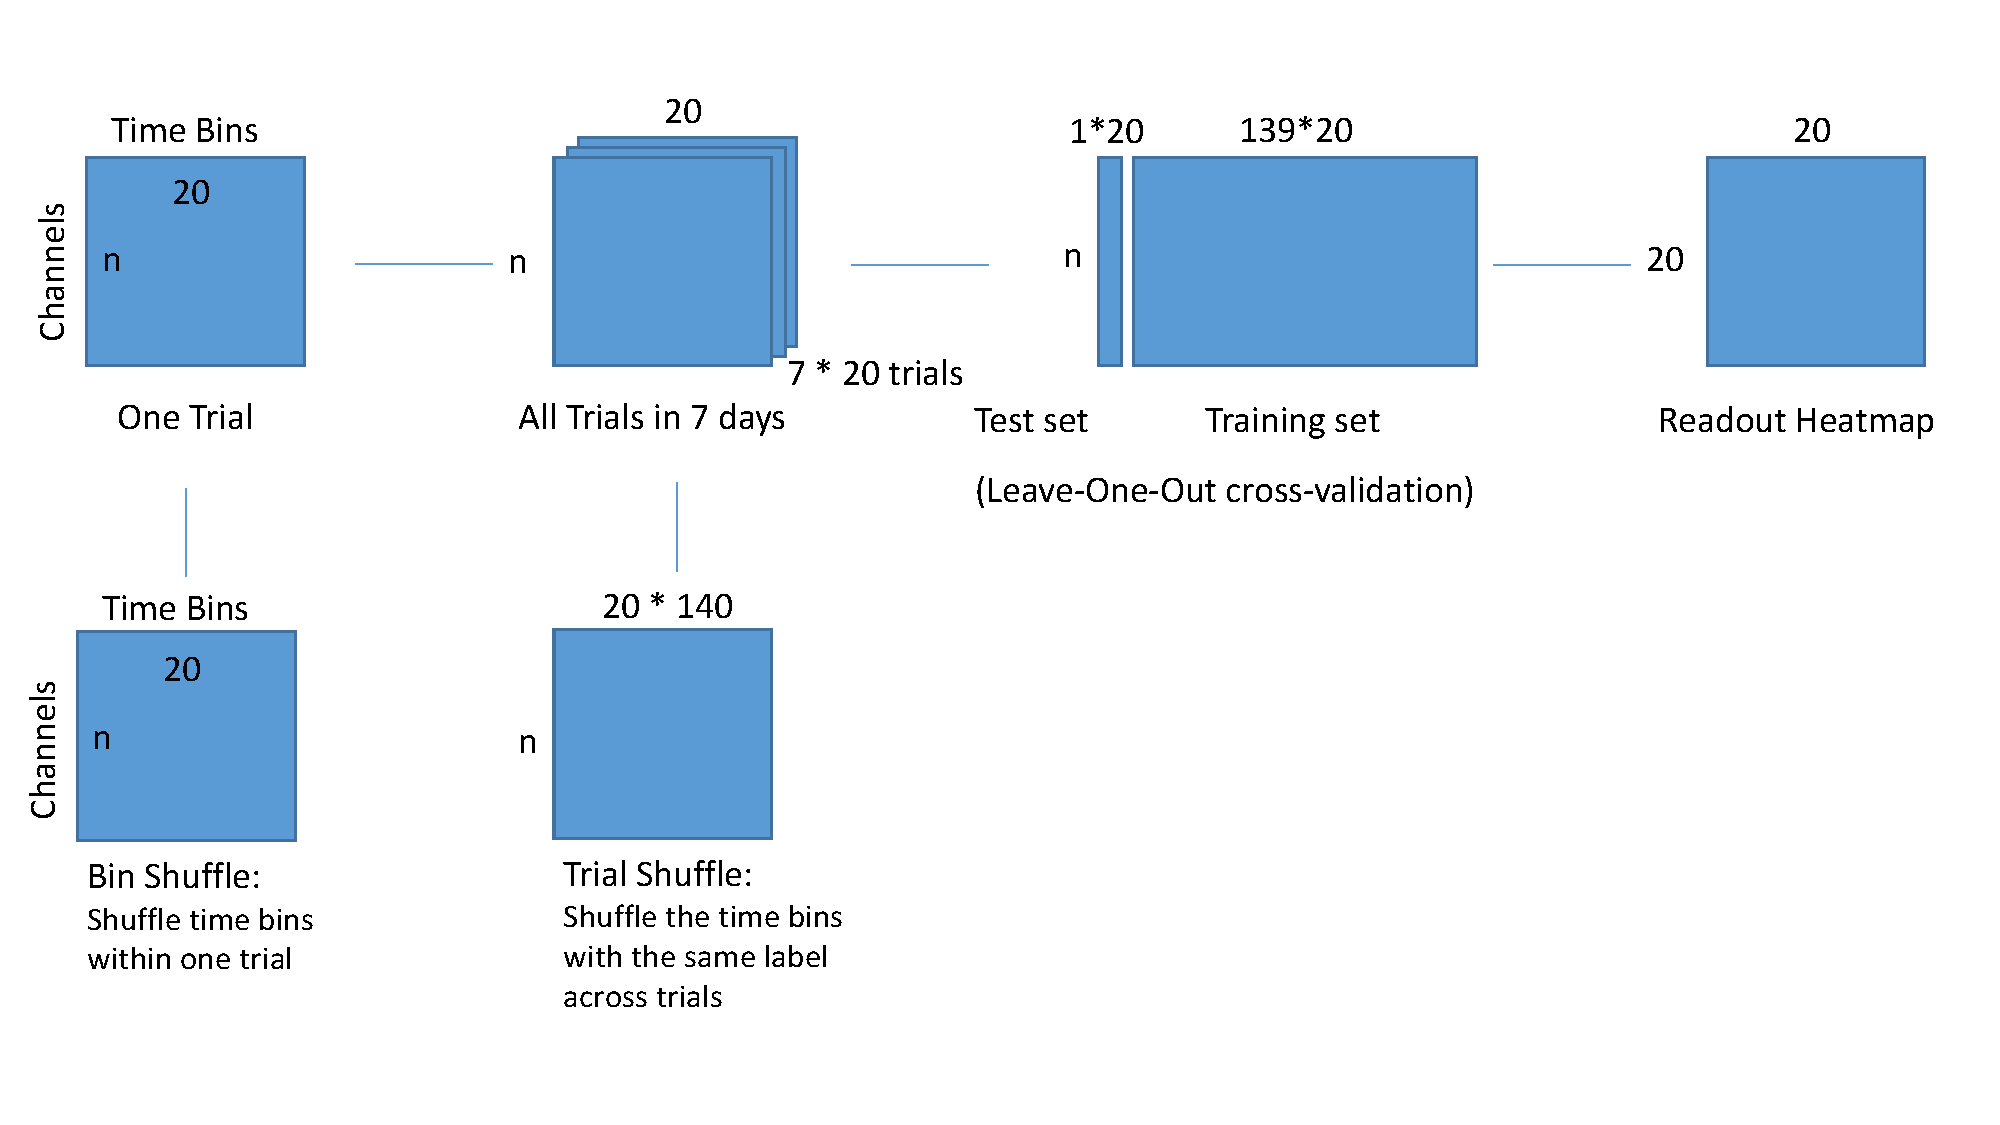
\includegraphics[width=\textwidth]{src/figures/svm_workflow.pdf}
    \caption{支持向量机分析的基本流程}
    \label{fig:svm_scheme}
\end{figure}

\subsubsection{分析用代码}
视觉刺激用代码如有需要, 请与本人或指导老师联系, 如理由正当合理将以邮件形式分享。
后续数据分析用Python代码可在\href{https://github.com/ZhangJiayiLab/EEGAnalysis/releases/tag/v1.0}{GitHub}获得。
